%! TeX program = lualatex
\documentclass[12pt,a4paper]{article}

\usepackage[nil]{babel}
\usepackage{unicode-math}
\usepackage[svgnames]{xcolor}
\usepackage{lmodern}
\usepackage{graphicx}
\usepackage{wrapfig}
\usepackage{float}
\usepackage{parskip}

\babelprovide[import=el, main, onchar=ids fonts]{greek} % can also do import=el-polyton
\babelprovide[import, onchar=ids fonts]{english}

\babelfont{rm}
          [Language=Default]{Liberation Sans}
\babelfont[english]{rm}
          [Language=Default]{Liberation Sans}
\babelfont{sf}
          [Language=Default]{Liberation Sans}
\babelfont{tt}
          [Language=Default]{Liberation Sans}

%Enter Title Here
 \title{Class-diagram-v1.0 \\ LibShare}
\author{\textbf{Ονόματα / ΑΜ / Έτος:} \\ Γρηγόρης Καπαδούκας / 1072484 / 4\textdegree \\ Χρήστος Μπεστητζάνος / 1072615 / 4\textdegree \\ Νικόλαος Αυγέρης / 1067508 / 5\textdegree \\ Περικλής Κοροντζής / 1072563 / 4\textdegree}

\begin{document}

\makeatletter
\begin{center}
	\LARGE{\@title} \\
	\pagebreak
    \begin{LARGE}\@author\end{LARGE} 
    \pagebreak
\end{center}

%Insert Body Here
\section{Σχήμα Class Diagram}

\begin{figure}[H]
	\makebox[\textwidth]{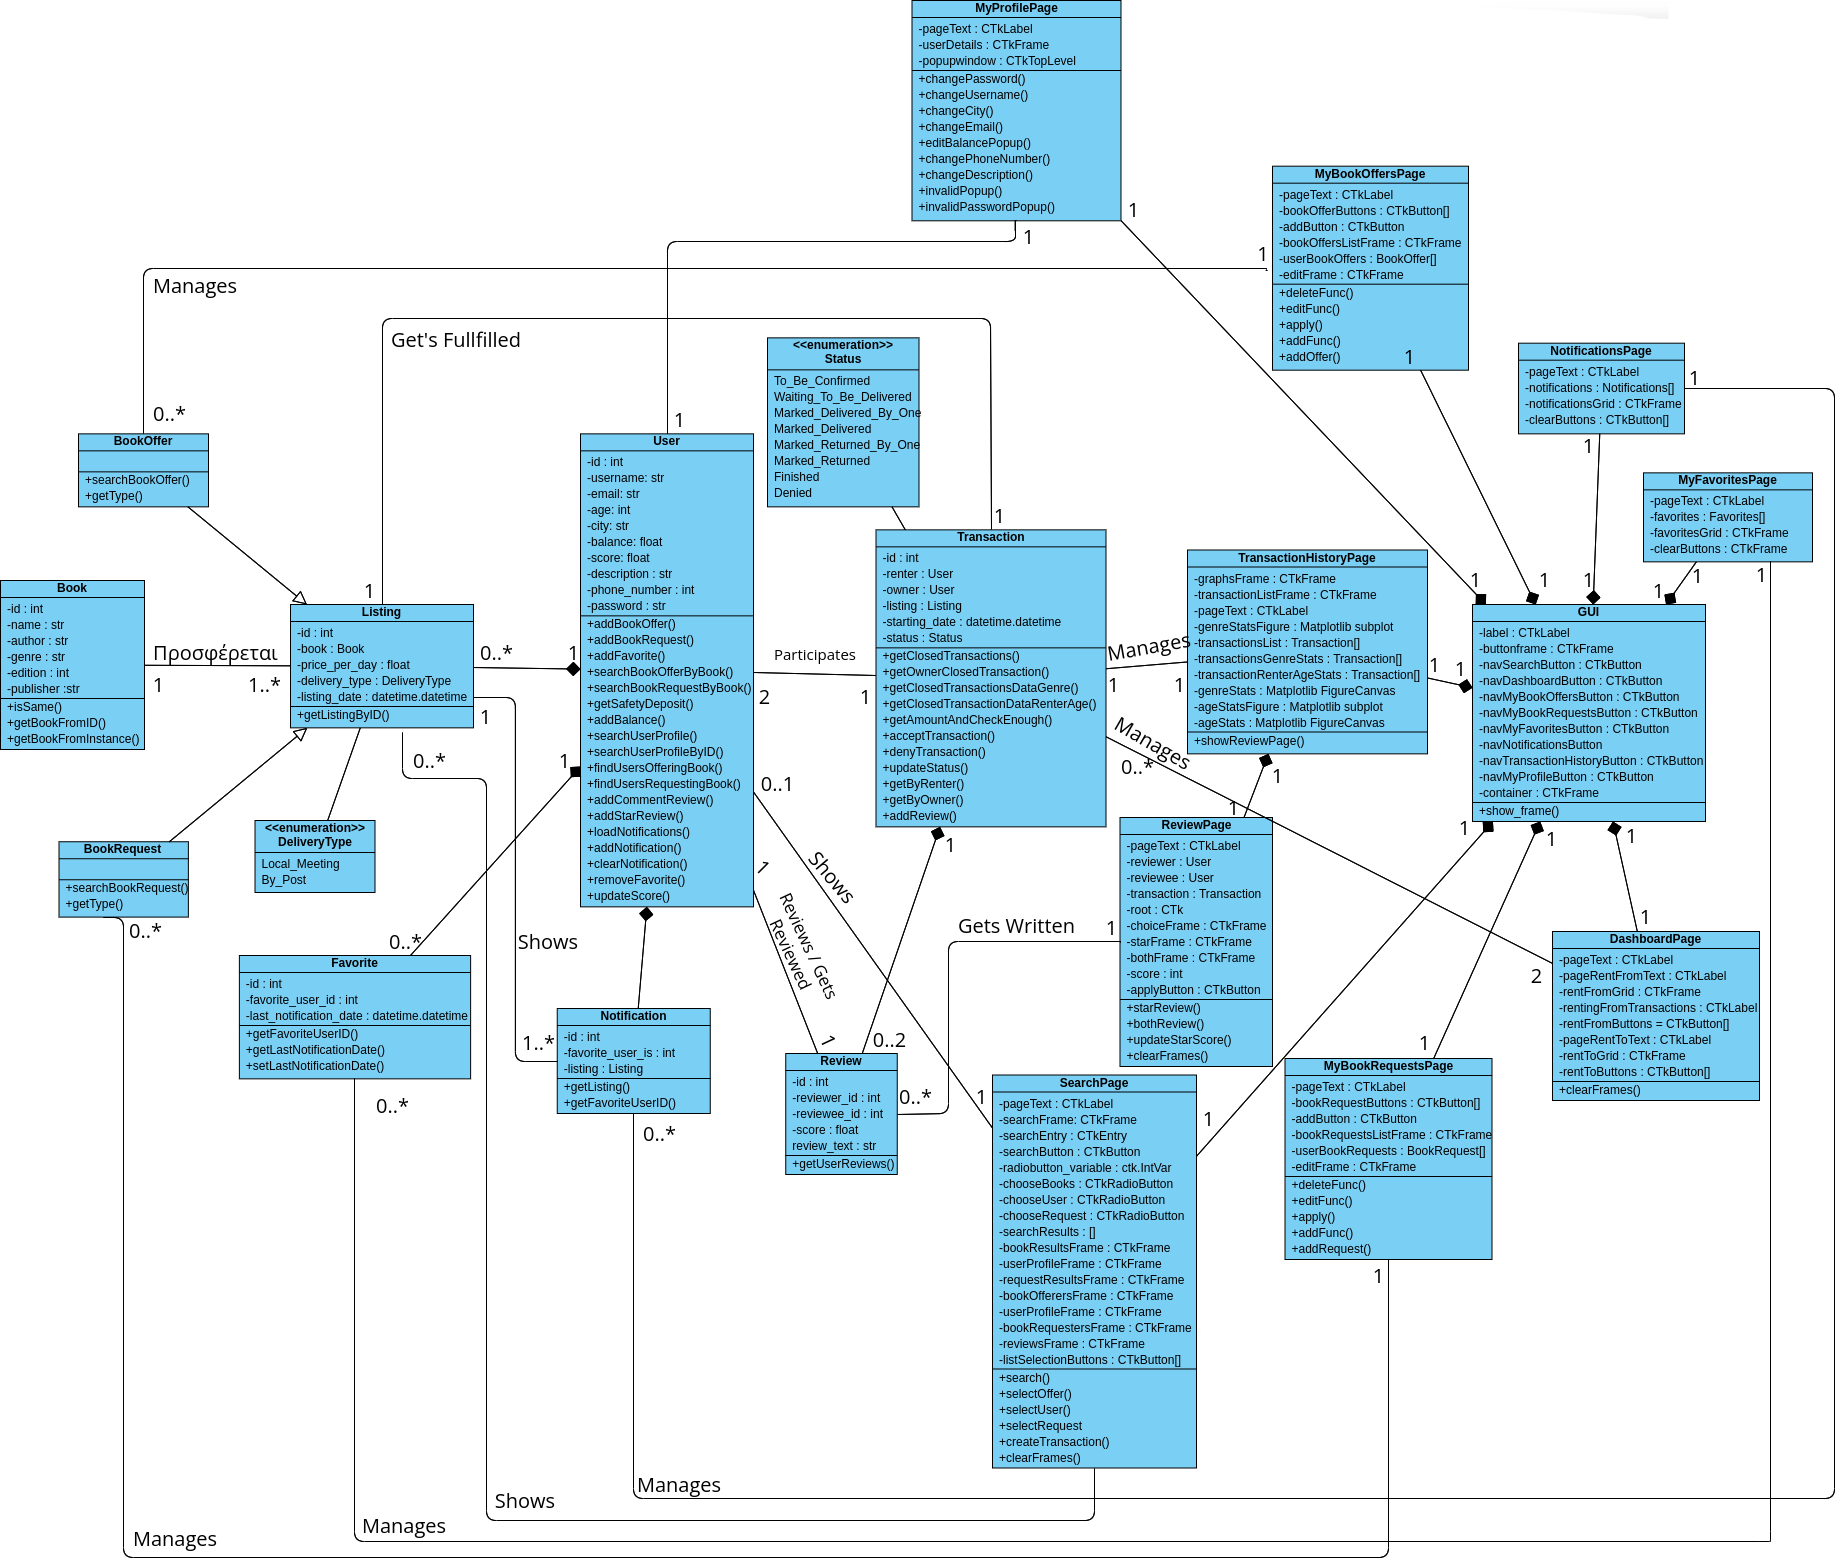
\includegraphics[width=\textwidth]{Class Diagram.png}}
	\caption{Σχήμα Class Diagram}
	\label{Σχήμα Class Diagram}
\end{figure}

\textbf{Σημειώσεις:}
\begin{itemize}
    \item Γνωρίζουμε ότι το σχήμα είναι πολύ μεγάλο και τα γράμματα φαίνονται μικρά, παρόλα αυτά έχουμε σιγουρευτεί ότι είναι ευδιάκριτα όταν γίνει zoom του αρχείου. Ταυτόχρονα παρέχεται και η εικόνα ξεχωριστά καθώς και το .vpd αρχείο του Visual Paradigm Online, που χρησιμοποιήθηκε για τη δημιουργία του σχήματος, στο GitHub της εργασίας.
    \item Για τις βασικές κλάσεις του class diagram (μη UI κλάσεις) έχουμε αποκρύψει τις περισσότερες getter και setter μεθόδους, ώστε να εξοικονομήσουμε χώρο. Κάθε getter και setter μας είναι public. Επίσης για τις κλάσεις του UI έχουμε αποκρύψει μερικά από τα πεδία που είναι στιγμιότυπα της CustomTKinter βιβλιοθήκης, δηλαδή UI elements, όταν περιοριζόμασταν από χώρο, δίνοντας μεγαλύτερη βάση στα κύρια UI elements και στα frames που περιέχουν τα elements αυτά.
\end{itemize}

\section{Σύντομη περιγραφή βασικών κλάσεων}

\subsection{User}
Ο κάθε χρήστης που είναι εγγεγραμμένος στην εφαρμογή μαζί με τα στοιχεία του. 
%Θα περιέχει βασικές πληροφορίες όπως όνομα, ηλικία, ποσό στον λογαριασμό του κλπ.

\subsection{Listing}
Οι καταχωρήσεις χρηστών αποτελούν τις "προσφορές" που αναρτούν στην εφαρμογή με σκοπό να γίνουν αποδεκτές από άλλους χρήστες. Συνδέεται με σχέση σύνθεσης με την κλάση "Χρήστης".
.
\subsection{BookOffer}
Αποτελεί τα βιβλία που προσφέρει ο χρήστης για ενοικίαση από άλλους χρήστες. Αποτελεί κλάση παιδί της κλάσης "Καταχώρηση".
%Έχει δεδομένα όπως: Ιδιοκτήτης βιβλίου (τύπου User), Βιβλίο (τύπου Book), τιμή κ.α.

\subsection{BookRequest}
Αποτελεί τις αιτήσεις βιβλίων που κάνει ο χρήστης. Δηλαδή αποτελεί αιτήσεις για βιβλία που δεν προσφέρονται ήδη από άλλο χρήστη, με σκοπό ο κάποιος που έχει το βιβλίο αλλά δεν το προσφέρει να αποδεχτεί την αίτηση και να νοικιάσει το βιβλίο στον χρήστη που το ζητάει, λαμβάνοντας μια επιπλέον ανταμοιβή. Αποτελεί κλάση παιδί της κλάσης "Καταχώρηση".
%Περιέχονται δεδομένα όπως: ο χρήστης που έκανε το request (τύπου User), το βιβλίο που ψάχνει (τύπου Book), την κατάσταση της αίτησης ("Ολοκληρωμένη" ή "Ενεργή") κ.α.

\subsection{Book}
Τα βιβλία που έχουν εισαχθεί στο σύστημα κατά την δημιουργία κάποιας καταχώρησης (είτε είναι διαθέσιμα για ενοικίαση είτε όχι).
%Περιέχονται βασικές πληροφορίες των βιβλίων όπως τίτλος, συγγραφέας, είδος (πχ φαντασίας), κατηγορία (πχ νουβέλα).

\subsection{Transaction}
Από τη στιγμή που κάποιος χρήστης κάνει αίτηση ενοικίασης ενός βιβλίου ή αίτηση εκπλήρωσης αίτησης δημιουργείται μια συναλλαγή. Αυτή έχει σκοπό να καταγράφει την κατάσταση της συναλλαγής, όπως αν είναι ενεργή, ακυρωμένη ή ολοκληρωμένη. Συνδέεται με σχέση συνάθροισης με την κλάση "Χρήστης".
%Περιέχει δεδομένα όπως τον ιδιοκτήτη του βιβλίου (τύπου user), τον ενοικιαστή (τύπου user) το βιβλίο (τύπου Listing) την κατάσταση (σε τι κατάσταση βρίσκεται η διαδικασία, π.χ. "Ολοκληρωμένη", "Αναμένεται αποστολή" κ.α) και Tracking Number στη περίπτωση που γίνεται ταχυδρομική συναλλαγή.

\subsection{Review}
Μετά την ολοκλήρωση κάθε συναλλαγής οι χρήστες μπορούν να εισάγουν αξιολόγηση για τον χρήστη με τον οποίο έκαναν την συναλλαγή (ιδιοκτήτη ή ενοικιαστή), μαζί με προαιρετικό σχόλιο. Αυτές οι κριτικές αποτελούν στιγμιότυπα κλάσης "Αξιολόγηση" και συνδέονται με την κλάση "Συναλλαγή" με σχέση σύνδεσης.


\subsection{Favorite}
Αποτελεί κλάση που καταγράφει χρήστες τους οποίους ένας χρήστης “ακολουθεί” (δηλαδή έχει προσθέσει στην λίστα αγαπημένων του). Συνδέεται με σχέση σύνθεσης με την κλάση "Χρήστης".
%Αποθηκεύεται ο χρήστης "αγαπημένος" και ο χρήστης που πρόσθεσε τον άλλον στη λίστα του.

\subsection{Notification}
Όταν ένας αγαπημένος χρήστης ενός άλλου χρήστη προσθέσει νέα καταχώρηση στην πλατφόρμα δημιουργείται μια ειδοποίηση για τον χρήστη, προσφέροντας έτσι τη δυνατότητα στους χρήστες να ενημερώνονται άμεσα για τις νέες καταχωρήσεις των "αγαπημένων" τους. Η ειδοποίηση αυτή είναι στιγμιότυπο της κλάσης "Ειδοποίηση", η οποία συνδέεται με σχέση σύνθεσης με την κλάση "Χρήστης".

\section{Σύντομη περιγραφή UI κλάσεων}

\subsection{GUI}
Η κλάση του GUI αποτελεί το κύριο παράθυρο του κώδικα και περιέχει πάνω το navigation bar. Επίσης περιέχεται ένα αρχικά κενό CTkFrame το container. Μέσω του navigation bar ο χρήστης μπορεί να φορτώσει στη σελίδα, το οποίο γίνεται μέσω της δημιουργίας στιγμιότυπου των υπολοίπων UI κλάσεων(εκτός του ReviewPage), οι οποίες UI κλάσεις κληρονομούν από το CTkFrame, και τη μετέπειτα αντικατάσταση του container με το CTkFrame που δημιουργείται, άρα φορτώνοντας τη σελίδα που θέλει κάθε φορά ο χρήστης κάτω από το navigation bar.

\subsection{SearchPage}
Αποτελεί την οθόνη αναζήτησης του χρήστη. Από εδώ μπορεί ο χρήστης να κάνει αναζήτηση για προσφορές βιβλίων, να προβάλλει ποιοι χρήστες προσφέρουν το βιβλίο αυτό, και να δημιουργήσει μια νέα συναλλαγή με αυτούς.

Επίσης μπορεί να αναζητήσει για άλλους χρήστες και να προβάλει το προφίλ και τα reviews τους, έχοντας και τη δυνατότητα για προσθήκη του χρήστη στη λίστα αγαπημένων τους.

Τέλος μπορεί να αναζητήσει και για αιτήσεις βιβλίων που είναι διαθέσιμες στη πλατφόρμα, να προβάλλει τους χρήστες που κάνουν αίτηση για το συγκεκριμένο βιβλίο και να κάνει συναλλαγή με αυτούς.

\subsection{DashboardPage}
Το DashboardPage αποτελεί την οθόνη όπου ο χρήστης βλέπει τις τρέχουσες συναλλαγές του. Από εδώ μπορεί να κάνει "Accept" ή "Deny" μια συναλλαγή, να κάνει δήλωση "Mark Possession" και "Mark Returned", αλλάζοντας κάθε φορά αντίστοιχα το status της συναλλαγής.

\subsection{MyBookOffersPage}
Η οθόνη όπου μπορεί ο χρήστης να προβάλλει τις προσφορές βιβλίων του, να προσθέσει και άλλες και να επεξεργαστεί ή να διαγράψει τις ήδη υπάρχουσες.

\subsection{MyBookRequestsPage}
Η οθόνη όπου μπορεί ο χρήστης να προβάλλει τις αιτήσεις βιβλίων του, να προσθέσει και άλλες και να επεξεργαστεί ή να διαγράψει τις ήδη υπάρχουσες.

\subsection{MyFavoritesPage}
Η οθόνη όπου μπορεί ο χρήστης να προβάλλει τη λίστα αγαπημένων του και να διαγράψει τυχόν χρήστες που δεν θέλει πλέον στη λίστα.

\subsection{NotificationsPage}
Η οθόνη όπου μπορεί ο χρήστης να προβάλλει τις ειδοποιήσεις που δημιουργούνται όταν οι αγαπημένοι του χρήστες προσθέτουν μια προσφορά βιβλίου ή μια αίτηση βιβλίου.

\subsection{TransactionHistoryPage}
H οθόνη όπου ο χρήστης προβάλλει το ιστορικό συναλλαγών του, προβάλλει στατιστικά για τα βιβλία και τις συναλλαγές όπου ήταν ο ίδιος ο ιδιοκτήτης και του δίνεται η δυνατότητα μετάβασης στην σελίδα που κάνει τις αξιολογήσεις των άλλων χρηστών.

\subsection{ReviewPage}
Αποτελεί μια ξεχωριστή σελίδα που δημιουργείται όταν το επιλέξει ο χρήστης στο TransactionHistoryPage και επιτρέπει στον χρήστη να προσθέσει αξιολόγηση χρήστες με τους οποίους έκανε συναλλαγή.

\subsection{MyProfilePage}
Αποτελεί την οθόνη όπου ο χρήστης προβάλλει τα στοιχεία του και τα επεξεργάζεται.

\section{Συμμετοχή και Ρόλοι στη Συγγραφή του Κειμένου}
\begin{enumerate}
	\item \textbf{Γρηγόρης Καπαδούκας:} Author
	\item \textbf{Περικλής Κοροντζής:} Author
    \item \textbf{Χρήστος Μπεστητζάνος:} Contributor
\end{enumerate}

\section{Αλλαγές από έκδοση σε έκδοση}

\subsection{Από έκδοση Domain-model v0.1 σε έκδοση Domain-model v0.2}
\begin{itemize}
    \item Σχεδίαση του Domain-model από την αρχή, μέσω του Visual Paradigm.
    \item Προσθήκη σωστών συσχετίσεων μεταξύ κλάσεων.
    \item Μετάφραση ονομάτων κλάσεων στα ελληνικά.
    \item Προσθήκη της κλάσης "Καταχώρηση" και ορισμός των "Προσφορά βιβλίου" και "Αίτηση βιβλίου" ως κλάσεις παιδιά της.
    \item Προσθήκη κλάσεων "Πόλη", "Ειδοποίηση", "Αγαπημένος χρήστης".
\end{itemize}

\subsection{Από έκδοση Domain-model v0.2 σε έκδοση Domain-model v0.3}
\begin{itemize}
    \item Προσθήκη επιπλέον συσχετίσεων μεταξύ κλάσεων.
    \item Προσθήκη στατικού μοντέλου attributes που προέκυψαν από τα Robustness Diagrams.
    \item Προσθήκη μεθόδων στις κλάσεις από το Sequence Diagram.
    \item Προσθήκη multiplicities of associations.
\end{itemize}

\subsection{Από έκδοση Domain-model v0.3 σε έκδοση Class-diagram v0.1}
\begin{itemize}
    \item Προσαρμογή ώστε τα ονόματα των κλάσεων, τα πεδία και οι μέθοδοι να αντιστοιχούν στον κώδικα Project-code v0.2
    \item Προσθήκη όλων των UI κλάσεων.
\end{itemize}

\subsection{Από έκδοση Class-diagram v0.3 σε έκδοση Class-diagram v1.0}
\begin{itemize}
    \item Προσαρμογή ώστε να υπάρχει αντιστοίχηση με το Project-code v1.0
    \item Προσθήκη βασικού σχολιασμού και για όλες τις UI κλάσεις.
\end{itemize}

\end{document}
